\documentclass[journal,10pt,twocolumn]{IEEEtran}
%

%\usepackage{graphicx}
%\usepackage{amssymb}
%\usepackage{relsize}
\usepackage[cmex10]{amsmath}
%\usepackage{amsthm}
\interdisplaylinepenalty=2500
%\savesymbol{iint}
%\usepackage{txfonts}
%\restoresymbol{TXF}{iint}
%\usepackage{wasysym}
\usepackage{amsthm}
\usepackage{mathrsfs}
\usepackage{txfonts}
\usepackage{stfloats}
\usepackage{float}
\usepackage{cite}
\usepackage{cases}
\usepackage{wrapfig}
\usepackage{subfig}
%\usepackage{xtab}
\usepackage{longtable}
\usepackage{multirow}
%\usepackage{algorithm}
%\usepackage{algpseudocode}
\usepackage{enumitem}
\usepackage{mathtools}
% \usepackage{iithtlc}
%\usepackage{stmaryrd}


%\usepackage{wasysym}
\DeclareMathOperator*{\Res}{Res}
%\renewcommand{\baselinestretch}{2}
\renewcommand\thesection{\arabic{section}}
\renewcommand\thesubsection{\thesection.\arabic{subsection}}
\renewcommand\thesubsubsection{\thesubsection.\arabic{subsubsection}}

\renewcommand\thesectiondis{\arabic{section}}
\renewcommand\thesubsectiondis{\thesectiondis.\arabic{subsection}}
\renewcommand\thesubsubsectiondis{\thesubsectiondis.\arabic{subsubsection}}


\begin{document}
%




\bibliographystyle{IEEEtran}

\title{Making an FM Transmitter}



\author{\IEEEauthorblockN{Varanasi Shashank}
\IEEEauthorblockA{ - ES16BTECH11025\\}
\and
\IEEEauthorblockN{Akshita Ramya}
\IEEEauthorblockA{ - ES16BTECH11012\\}
\and
\IEEEauthorblockN{Bhanu Prakash}
\IEEEauthorblockA{ - ES16BTECH11022\\}
\and
\IEEEauthorblockN{Roshni Pande}
\IEEEauthorblockA{ - EE16BTECH11032} % <-this % stops a space
}

\maketitle
\IEEEpeerreviewmaketitle

\section*{Introduction}
FM broadcasting is a method of radio broadcasting using frequency modulation (FM) technology. FM broadcasting is capable of better sound quality than AM broadcasting, the chief competing radio broadcasting technology, so it is used for most music broadcasts. FM radio stations use the VHF frequencies. The term FM band describes the frequency band in a given country which is dedicated to FM broadcasting.


%\newpage
\section*{Project Details}
The radio we have worked on is a miniature FM Transmitter, the transmission frequency of which range between 80MHz and 100MHz. Transmissions in this range can be picked up by any standard receiver. It has a range of around 400m. 
\begin{figure}[H]
\centering
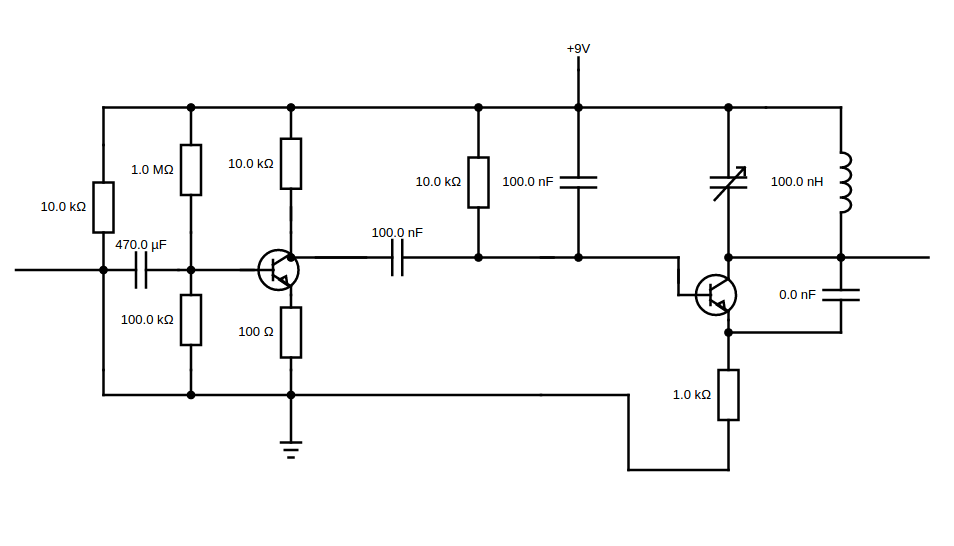
\includegraphics[width=3.5in]{picture.png}
\caption{Circuit diagram}
\end{figure}


The input is given from the left. The first capacitor filters the DC component of the input. This is passed through a transistor which amplifies the filtered signal. The DC components are filtered once again, and this signal is then modulated with the carrier signal (generated from the LC oscillator) at the second transistor. This signal is transmitted through the antenna.

\section*{Components}
\begin{description}
	\item[$\bullet$ 10K ohm Resistors] - 3
	\item[$\bullet$ 1000K ohm Resistors] - 1
	\item[$\bullet$ 10M ohm Resistors] - 1
	\item[$\bullet$ 100 ohm Resistors] - 1
	\item[$\bullet$ 1K ohm Resistors] - 1
	\item[$\bullet$ 0.1 microFarads Capacitor] - 2
	\item[$\bullet$ 0.01 microFarads Capacitor] - 2
	\item[$\bullet$ 4.7 picoFarads Capacitor] - 1
	\item[$\bullet$ ~2.2 picoFarads Variable Capacitor] - 2
	\item[$\bullet$ 2N3904 Transistors] - 2
	\item[$\bullet$ 0.22 microHenry Inductor] - 2

\end{description}

\section*{Working Of The Circuit}
In the right we have a tuning amplifier, i.e. an LC circuit which produces the carrier wave and a transistor. 
The message signal is modulated here at the tuning amplifier and transmitted through the antenna which here is a long single strand wire.
The capacitors (except the variable the capacitance) filter out the DC components from the wave if any present.
For our circuit, the carrier wave frequency is 105.3MHz, as is predicted by
\begin{equation}
\omega = 1 \div  \sqrt{LC}
\end{equation}
if the input signal is \begin{equation*} x_{m}(t), \end{equation*} then the modulated output is given by -
\begin{equation}
y(t) = A_{c} cos \big(2\pi  \int_0^t  f( \lambda ) d\lambda\big),
\end{equation}
where \begin{equation*}f(\lambda)\end{equation*} is the instantaneous frequency, which is given by - 
\begin{equation}
\int_0^t f(\lambda) d\lambda = 2\pi f_{c}t + 2\pi f_{\Delta} \int_0^t x_{m}(\tau) d\tau 
\end{equation}
We used our mobile phones to recieve the signal by tuning it the above frequency.
The range was about 500m. We observed that we had interference from the other transmitters. We also observed that if we cannot transmit very high frequencied message signals. The noise generated by the circuit itself was also large, and due to the sensitivity of the variable capacitor, we noticed large carrier frequency jumps. This can be reduced if special capacitors and inductors of much lower values are used, to make the circuit using as few components as possible.

\end{document}


